% il existe plusieures classes de documents
% pour des documents plus longs, vous pouvez utiliser
% book ou report
\documentclass[10pt]{article} 

\usepackage[a4paper,  fancysections,  titlepage]{polytechnique}
\usepackage[english]{babel}
\usepackage[T1]{fontenc}
\usepackage[hidelinks]{hyperref}
\usepackage{amsmath, amssymb}
\usepackage{pdfpages}
\usepackage{setspace}
\usepackage{graphicx}
\usepackage{booktabs}
\usepackage{subcaption}
\usepackage{xcolor}
\usepackage{float}

\setlength{\parskip}{0.7em}
\setstretch{1}

\newcommand{\code}[1]{\mbox{\ttfamily\detokenize{#1}}}
\newcommand{\todo}[1]{\textcolor{red}{\textbf{#1}}}

\author{Nathan Duboisset}
\date{\today}
\title{Image Synthesis Project}
\subtitle{Lightcuts and Stochastic Lightcuts — Polytechnique, February 2026}


\begin{document}

\maketitle
\tableofcontents
\newpage

% -----------------------------------------------------------------------
\section{Introduction}
% -----------------------------------------------------------------------

This project implements three many-light rendering algorithms on top of a WebGPU
ray-tracer built during the course assignments:
\textbf{Lightcuts}~\cite{walter2005lightcuts},
\textbf{Stochastic Lightcuts}~\cite{yuksel2019slc,yuksel2020slc}, and a
\textbf{tile-precomputed variant} inspired by real-time stochastic lightcuts~\cite{lin2020realtime}.

The test scene is a planar floor with a ram mesh, shaded with a Cook-Torrance
microfacet BRDF.
To study the algorithms in isolation, the scene is lit by \textbf{1600 point lights
arranged in a panel above the objects} rather than full VPLs — this keeps the light
count fixed and makes timing differences and visual artefacts clearly observable.
All algorithms run in WGSL compute shaders; the tree data structures are built on
the CPU and uploaded as GPU storage buffers.

% -----------------------------------------------------------------------
\section{Lightcuts}
% -----------------------------------------------------------------------

\subsection{Implementation}

Lightcuts~\cite{walter2005lightcuts} clusters lights into a binary tree and greedily
selects a per-pixel \emph{cut} of $K$ nodes, evaluating only one representative per
node instead of all $n$ lights.

\paragraph{Tree construction (\code{src/lightcutTree.ts}).}
Nodes are merged bottom-up with a priority queue (\code{js-priority-queue}) using:
\[
  c(A,B) = \|\mathbf{p}_A - \mathbf{p}_B\|^2 + \mathrm{vol}(\mathrm{AABB}(A \cup B))
\]
Each node stores an intensity-weighted representative and union AABB, serialised into
16-float structs uploaded to binding~8.

\paragraph{GPU cut construction (\code{computeRadianceLightcuts} in \code{shaders.wgsl}).}
Each shader invocation iteratively splits the highest-error node ($K_{\max}=32$) using:
\[
  \varepsilon(v,\mathbf{x}) = \frac{I_v \cdot \mathrm{diag}(v)}{\|\mathbf{x}-\mathbf{p}_v\|^3}
\]
Each final cut node contributes one BRDF evaluation and one shadow ray.

\subsection{Results}

\begin{figure}[H]
  \centering
  \begin{subfigure}[b]{0.48\linewidth}
    \includegraphics[width=\linewidth]{results/ramexamplelightcuts1600_16.png}
    \caption{Lightcuts render — 1600 lights, $K=32$.}
    \label{fig:lc}
  \end{subfigure}
  \hfill
  \begin{subfigure}[b]{0.48\linewidth}
    \includegraphics[width=\linewidth]{results/ligthcuttreelastrank.png}
    \caption{Lightcut tree — deepest level bounding boxes.}
    \label{fig:lctree}
  \end{subfigure}
  \caption{Lightcuts output and tree visualisation.}
\end{figure}

\begin{figure}[H]
  \centering
  \begin{subfigure}[b]{0.48\linewidth}
    \includegraphics[width=\linewidth]{results/lightcuttreesmallrank.png}
    \caption{Shallow cut.}
  \end{subfigure}
  \hfill
  \begin{subfigure}[b]{0.48\linewidth}
    \includegraphics[width=\linewidth]{results/lightcuttreebigrank.png}
    \caption{Deeper cut.}
  \end{subfigure}
  \caption{Tree visualisation at two depths — AABB bounding boxes rendered in a separate canvas.}
  \label{fig:lctrees}
\end{figure}

% -----------------------------------------------------------------------
\section{Stochastic Lightcuts}
% -----------------------------------------------------------------------

\subsection{Implementation}

Stochastic Lightcuts~\cite{yuksel2019slc} keeps the same cut but replaces the
deterministic sum with a Monte Carlo estimator: for each cut node, one leaf is
importance-sampled and its contribution rescaled by the inverse probability.

\paragraph{HIS — \code{selectLight()} in \code{shaders.wgsl}.}
The traversal weight at each node is:
\[
  w(v) =
  \begin{cases}
    I_v / d_{\min}^2 & d_{\min} > \mathrm{diag}(v) \\
    I_v              & \text{otherwise}
  \end{cases}
\]
biasing toward nearby bright clusters; the sampled leaf contributes $f(\ell)\cdot V(\ell)/p$.

\paragraph{Temporal accumulation.}
The frame counter seeds a per-pixel PCG hash for independent samples each frame.
Frames are accumulated additively and divided by the pass count.
Figures~\ref{fig:slc16} and~\ref{fig:slc64} compare 16 and 64 passes.

\subsection{Results}

\begin{figure}[H]
  \centering
  \begin{subfigure}[b]{0.48\linewidth}
    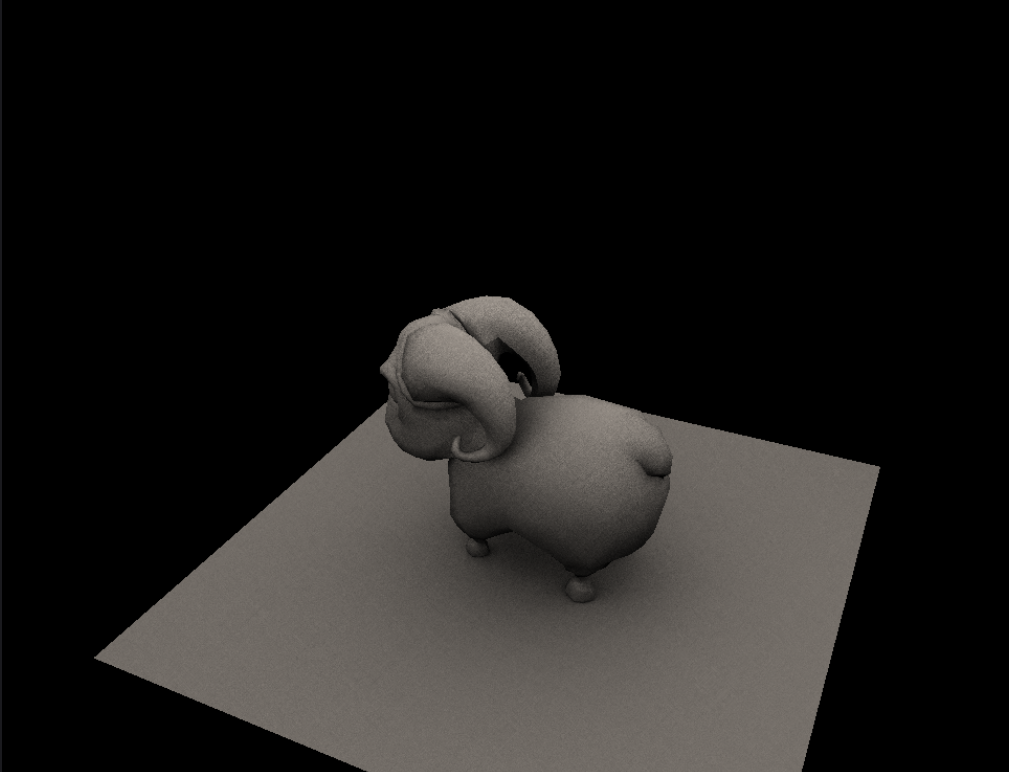
\includegraphics[width=\linewidth]{results/ramexamplestochasticlightcuts1600_16acc.png}
    \caption{16 accumulation passes.}
    \label{fig:slc16}
  \end{subfigure}
  \hfill
  \begin{subfigure}[b]{0.48\linewidth}
    
\includegraphics[width=\linewidth]{results/ramexamplestochasticlightcuts1600_64acc.png}
    \caption{64 accumulation passes.}
    \label{fig:slc64}
  \end{subfigure}
  \caption{Stochastic Lightcuts — 1600 lights, $K=32$, increasing accumulation.}
\end{figure}

% -----------------------------------------------------------------------
\section{Tile-Precomputed Stochastic Lightcuts}
% -----------------------------------------------------------------------

\subsection{Implementation}

Per-pixel cut construction is the dominant cost of Stochastic Lightcuts.
Following Lin \& Yuksel~\cite{lin2020realtime}, one cut is precomputed per screen tile
on the CPU (\code{buildCutsForTiles} in \code{src/lightcutTree.ts}): a ray through the
tile centre gives a representative world position; a max-heap builds a cut of up to $K$
nodes in $O(K\log n)$ and packs it into a flat \code{u32} buffer (stride $K+1$,
binding~9) uploaded before each frame.

On the GPU (\code{computeRadianceRealtimeStochasticLightcuts}), each pixel looks up
its tile cut with a single integer division and runs HIS only.
\code{selectLightRT()} uses the average of $p_{\min}$/$p_{\max}$ bounds so one cut
serves every pixel in the tile.

The method is not truly real-time in a browser (CPU build + JS upload add latency),
but the in-shader cost is noticeably lower than per-pixel cut construction
(Table~\ref{tab:perf}).

% -----------------------------------------------------------------------
\section{Results and Performance}
% -----------------------------------------------------------------------

\subsection{Performance}

All timings are wall-clock averages on a \todo{GPU model}, 1600 lights, $K=32$.

\begin{table}[H]
  \centering
  \caption{Average render time per frame — 1600 point lights, ram scene.}
  \label{tab:perf}
  \begin{tabular}{lrr}
    \toprule
    \textbf{Method} & \textbf{ms / frame} & \textbf{Notes} \\
    \midrule
    Brute-force RT               & \todo{XX} & reference, \todo{N} passes \\
    Lightcuts ($K=32$)           & \todo{XX} & single pass, clean         \\
    Stochastic LC ($K=32$)       & \todo{XX} & per pass, \todo{N} to converge \\
    Tile-precomputed SLC         & \todo{XX} & per pass, CPU upload incl. \\
    \bottomrule
  \end{tabular}
\end{table}

% -----------------------------------------------------------------------
\section{Conclusion}
% -----------------------------------------------------------------------

Three many-light algorithms were implemented in WebGPU/WGSL on top of the course
ray-tracer.
Lightcuts delivers a clean image in a single pass at a fraction of the brute-force
cost.
Stochastic Lightcuts is faster per frame and converges through temporal accumulation.
The tile-precomputed variant further reduces in-shader cost, validating the Lin \&
Yuksel 2020 approach even within the constraints of a browser runtime.
An interactive UI allows direct comparison of all three methods alongside a
lightcut tree visualisation.

% -----------------------------------------------------------------------
\bibliographystyle{plain}
\begin{thebibliography}{9}

\bibitem{walter2005lightcuts}
B.~Walter, S.~Fernandez, A.~Arbree, K.~Bala, M.~Donikian, D.~P.~Greenberg.
\newblock Lightcuts: A scalable approach to illumination.
\newblock \textit{ACM SIGGRAPH 2005 Papers}, pp.~1098--1107, 2005.

\bibitem{yuksel2019slc}
C.~Yuksel.
\newblock Stochastic Lightcuts.
\newblock \textit{High-Performance Graphics (HPG)}, 2019.
\newblock Wolfgang Stra{\ss}er Best Paper Award.

\bibitem{yuksel2020slc}
C.~Yuksel.
\newblock Stochastic Lightcuts for Sampling Many Lights.
\newblock \textit{IEEE Transactions on Visualization and Computer Graphics}, 2020.

\bibitem{lin2020realtime}
D.~Lin, C.~Yuksel.
\newblock Real-Time Stochastic Lightcuts.
\newblock \textit{Proc. ACM Comput. Graph. Interact. Tech.\ (I3D 2020)}, 3(1), 2020.
\newblock Best Paper Award.

\end{thebibliography}

\end{document}
